\section{Evaluation}
\label{sec:evaluation}
The evaluation is intended to answer the following questions -- \ca can we detect failures~\ie separate faulty PIR sensors from working ones? and \cb what can we learn about the failure? In other words, can we perform diagnosis that can aid in replacing or repairing the sensor? We answer these questions in practical deployments, %
each consisting of the following stages:

\ca {\bfseries Stage I: Failure Detection} The goal of this stage is to isolate defective, faulty sensors from functional, working sensors. Note that we do not diagnose the failure in this stage \ie the sensors deemed faulty could be so due to multiple, as yet unknown reasons.\\
\hspace*{2ex}\cb {\bfseries Stage II: Failure Diagnosis} In this stage, we diagnose the failure by mapping it to the taxonomy defined in \S\ref{subsec:taxonomy}. Using the taxonomy as a reference, we seek to conclude whether it is the lens, pyroelectric or electronics subsystem that contains the failure.\\
\hspace*{2ex}\cc {\bfseries Stage III: Fine-Grained Fault Analysis} In this stage, we learn details about the failure as precisely as possible. \Eg if we attribute a fault to be Class III failure, we seek to narrow it down to see if it is due to deposition of dust or paper on the lens.

\subsection{Real-world Deployments}
\label{subsec:deployment}


We performed the following \emph{deployments across multiple scenarios and geographic locations,~\viz}  
\ca in the elevator of a building (\S\ref{subsubsec:elevator}), 
\cb in the lobby of a university building (\S\ref{subsubsec:lobby}), \cc in a Starbucks coffee shop (\S\ref{subsubsec:starbucks}), and \cd in a cafeteria (\S\ref{subsubsec:cafeteria}) (India).
The different deployment scenarios \ca -- \cc are shown in {\bfseries Fig.~\ref{fig:pir_deployment_scenario}}, and aim to capture diverse environmental conditions and challenges (heat, dust, humidity~\etc). 
We used 15 sensors in total across all our deployments comprising of 5 working sensors and 2 faulty sensors per class. A combination of these was used in each of our deployments. In each of these deployments, we followed the pre-deployment process, as mentioned in \S\ref{sebsec:pre_deploy}, where different types of faulty sensors were deployed for a week to collect its \aout and \cout. This pre-deployment is a one-time process to calculate different time and frequency domain characteristics capturing the physics of \aout. A subset of these sensors used in the pre-deployment was randomly picked in each of the deployments.
These sensors were deployed (\textbf{Fig.~\ref{fig:pir_sensor_failure_photographs}}) %
over a duration of 3 months and collected data both during times of low occupancy (weekends, late nights) and high occupancy (weekdays, working hours). Note that no auxiliary private data such as audio or video were captured during these deployments. 

\begin{figure}[t!]
	\centering
	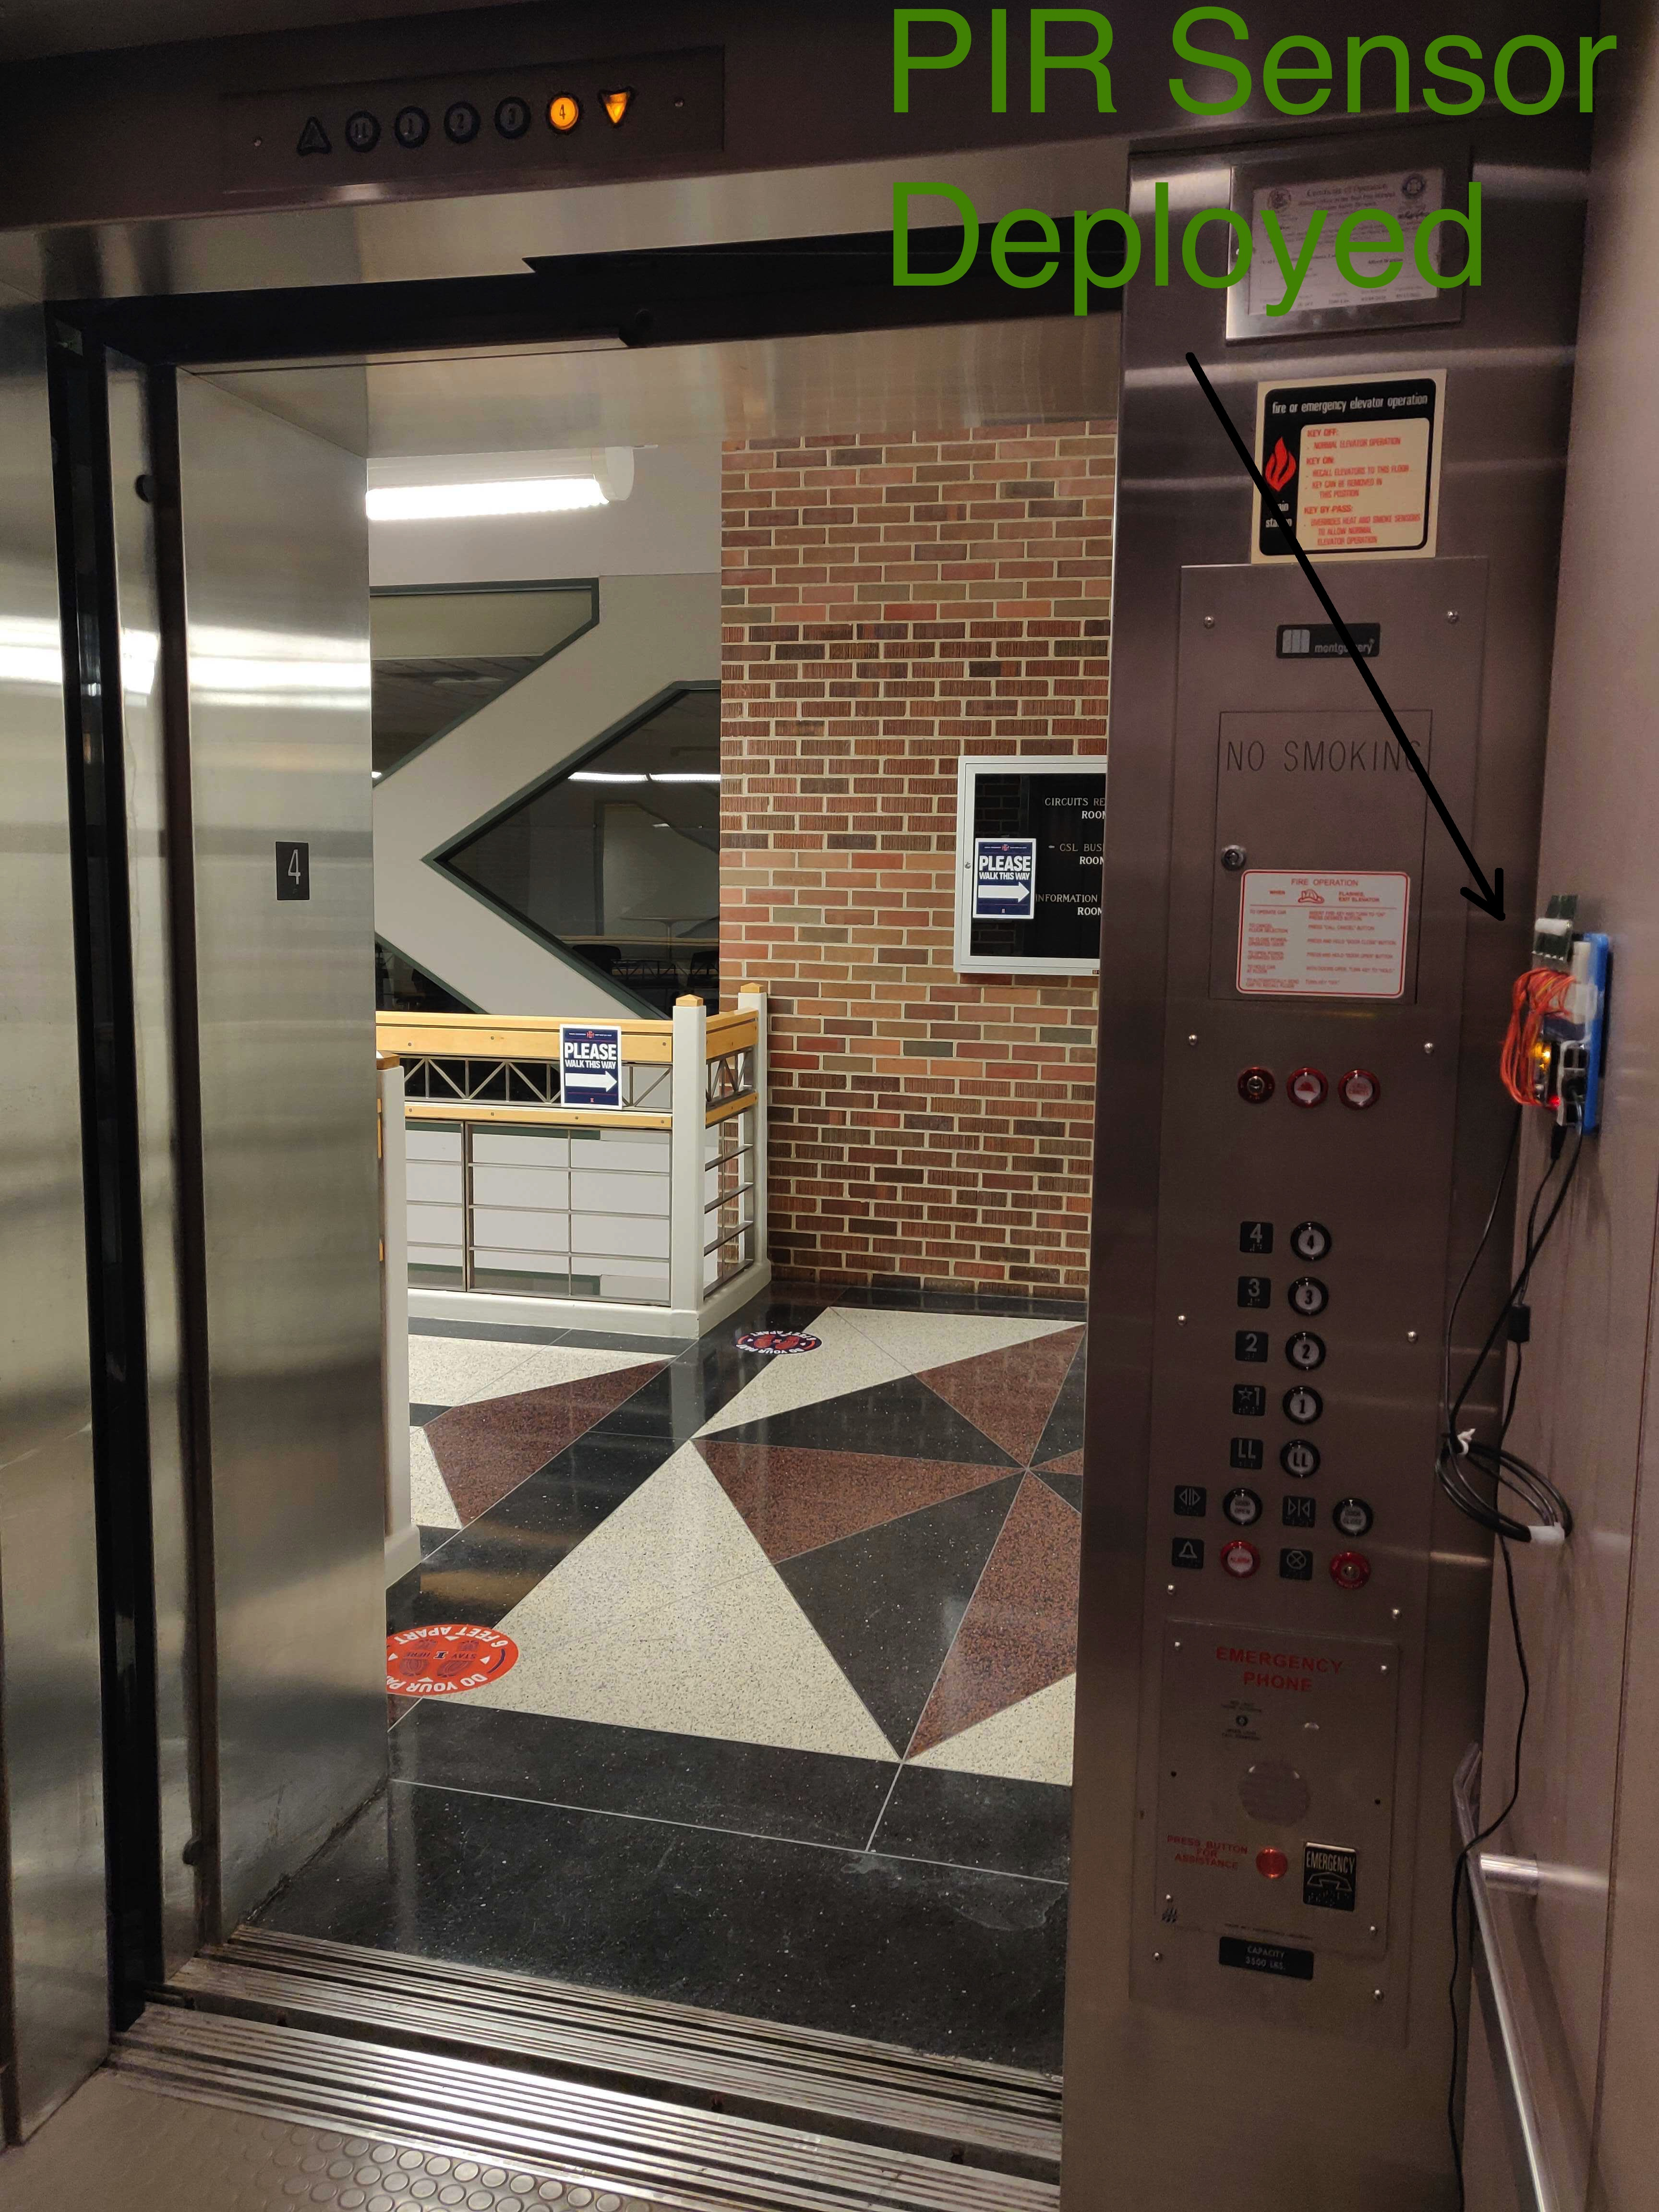
\includegraphics[width=0.3\textwidth, height=1.33in]{figures/deployment/elevator/Elevator-jpg.jpg}
	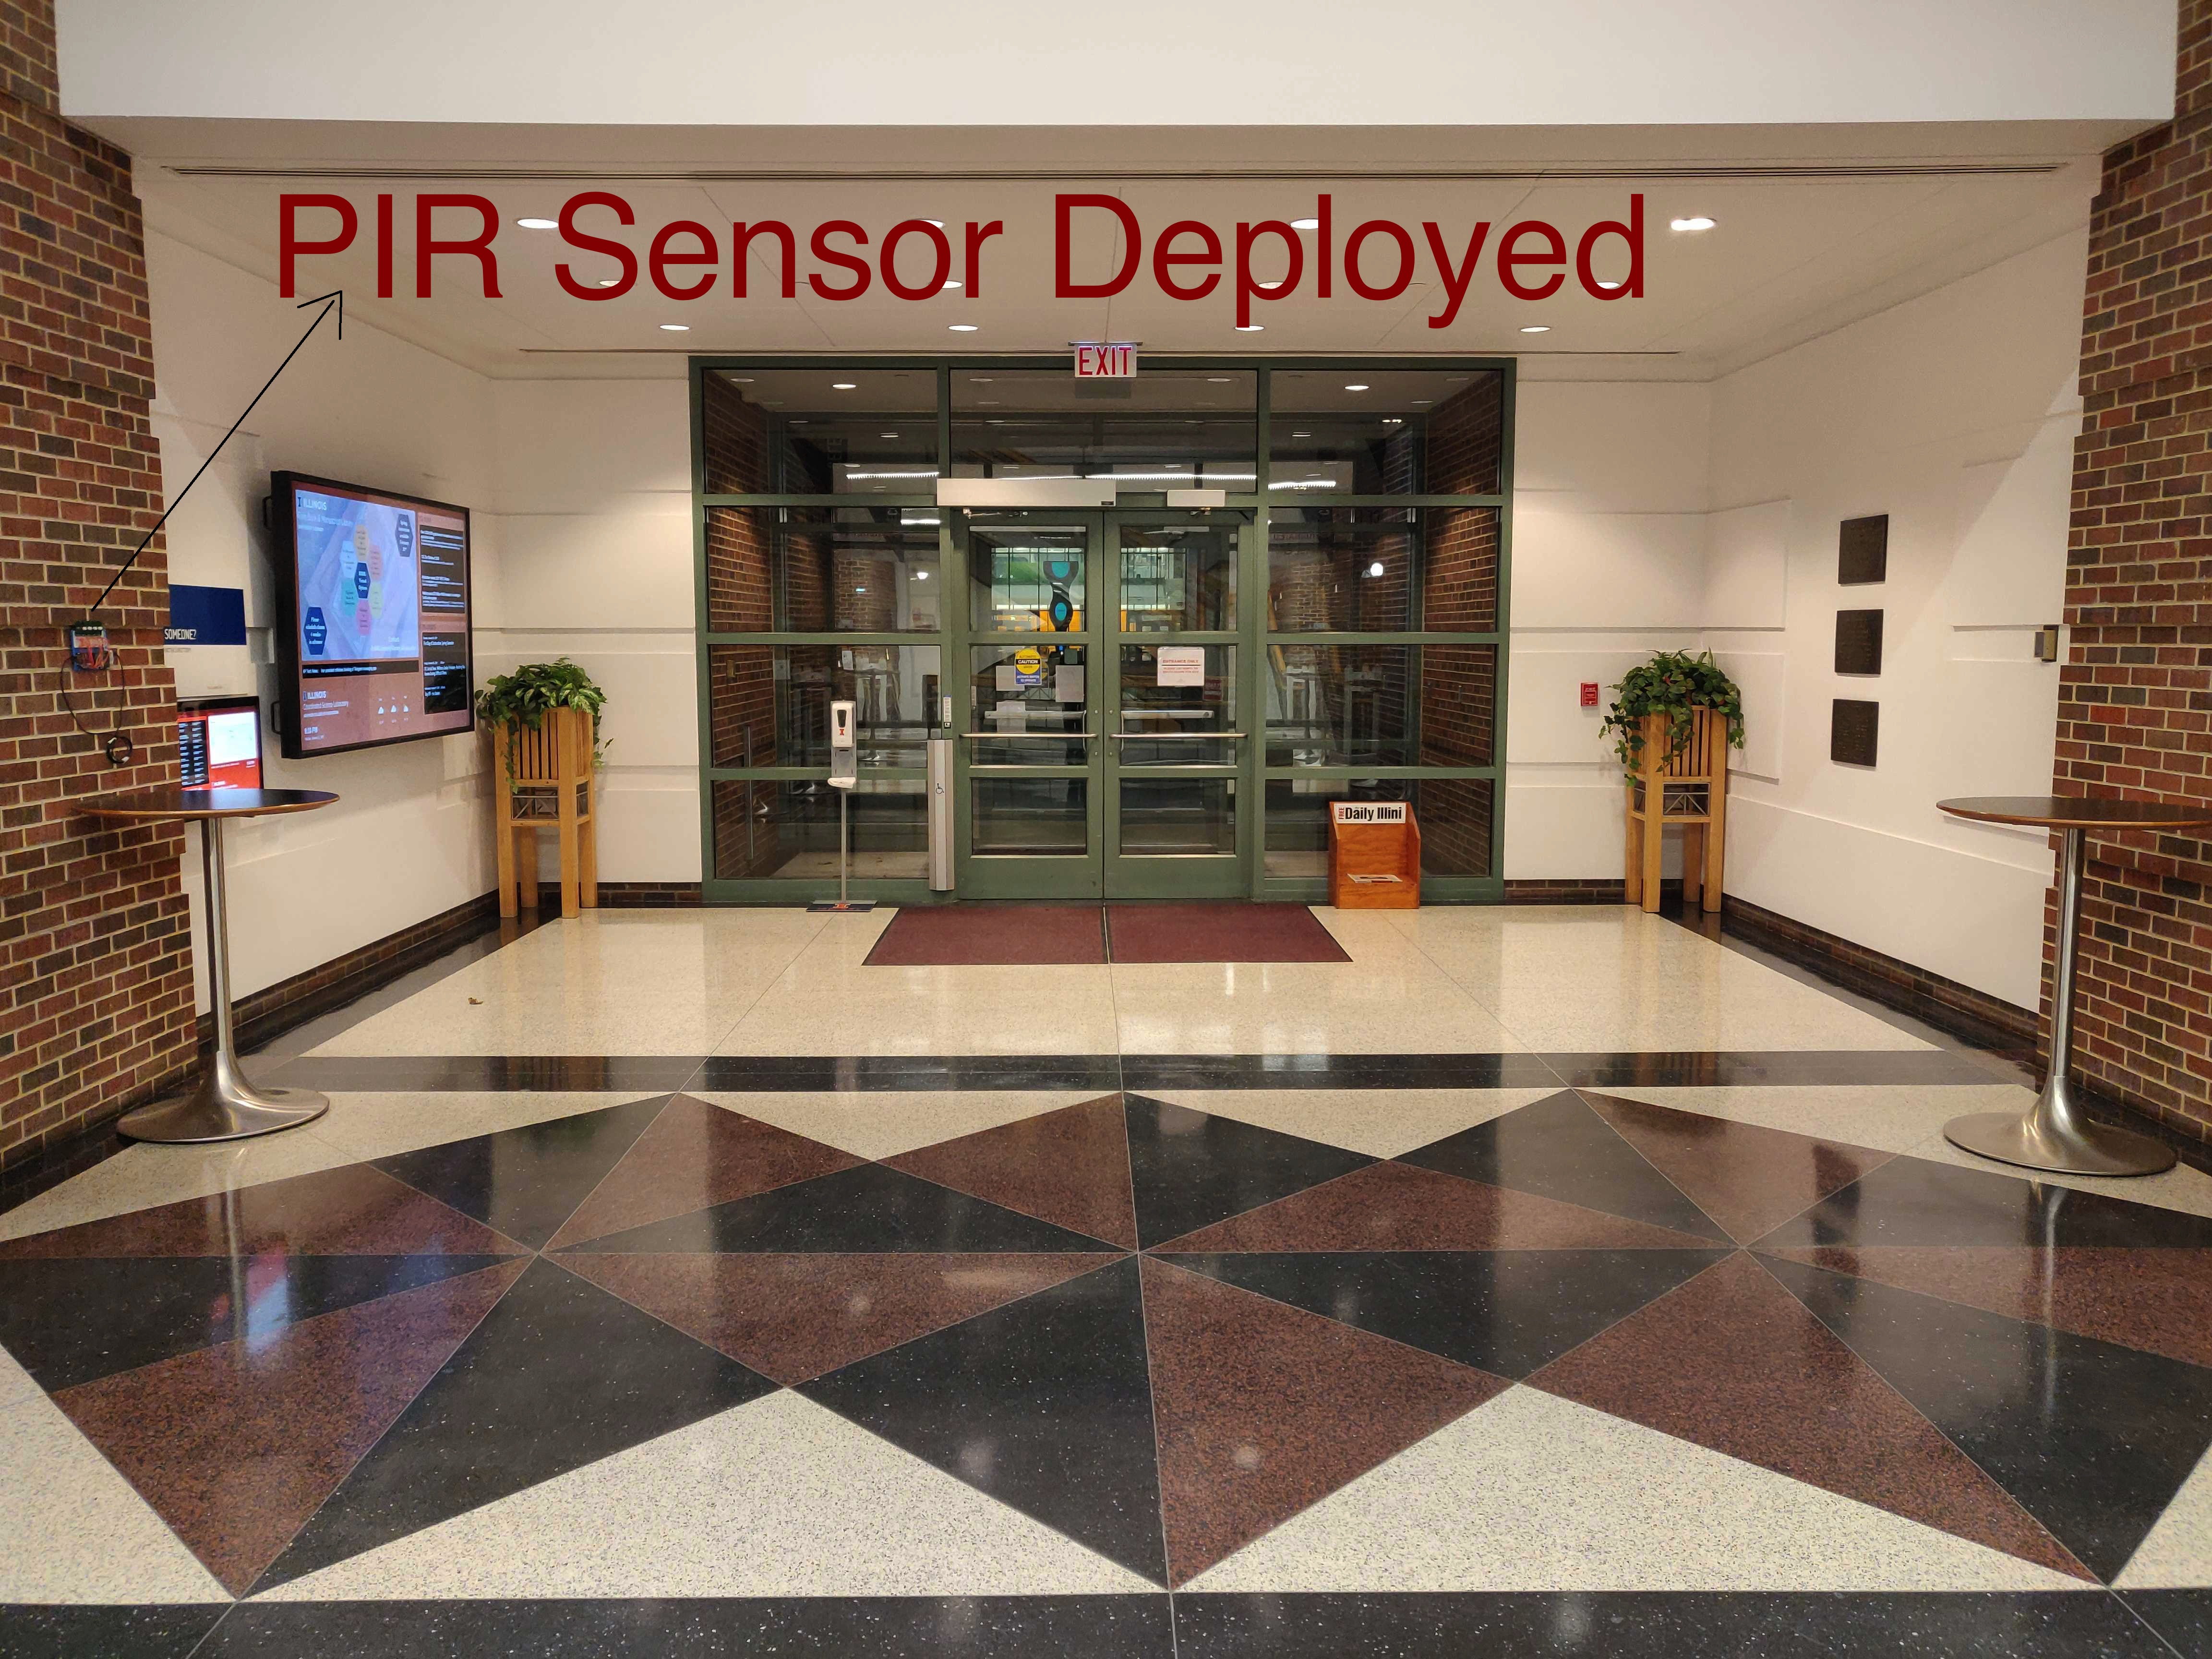
\includegraphics[width=0.3\textwidth]{figures/deployment/lobby/lobby.jpg}
	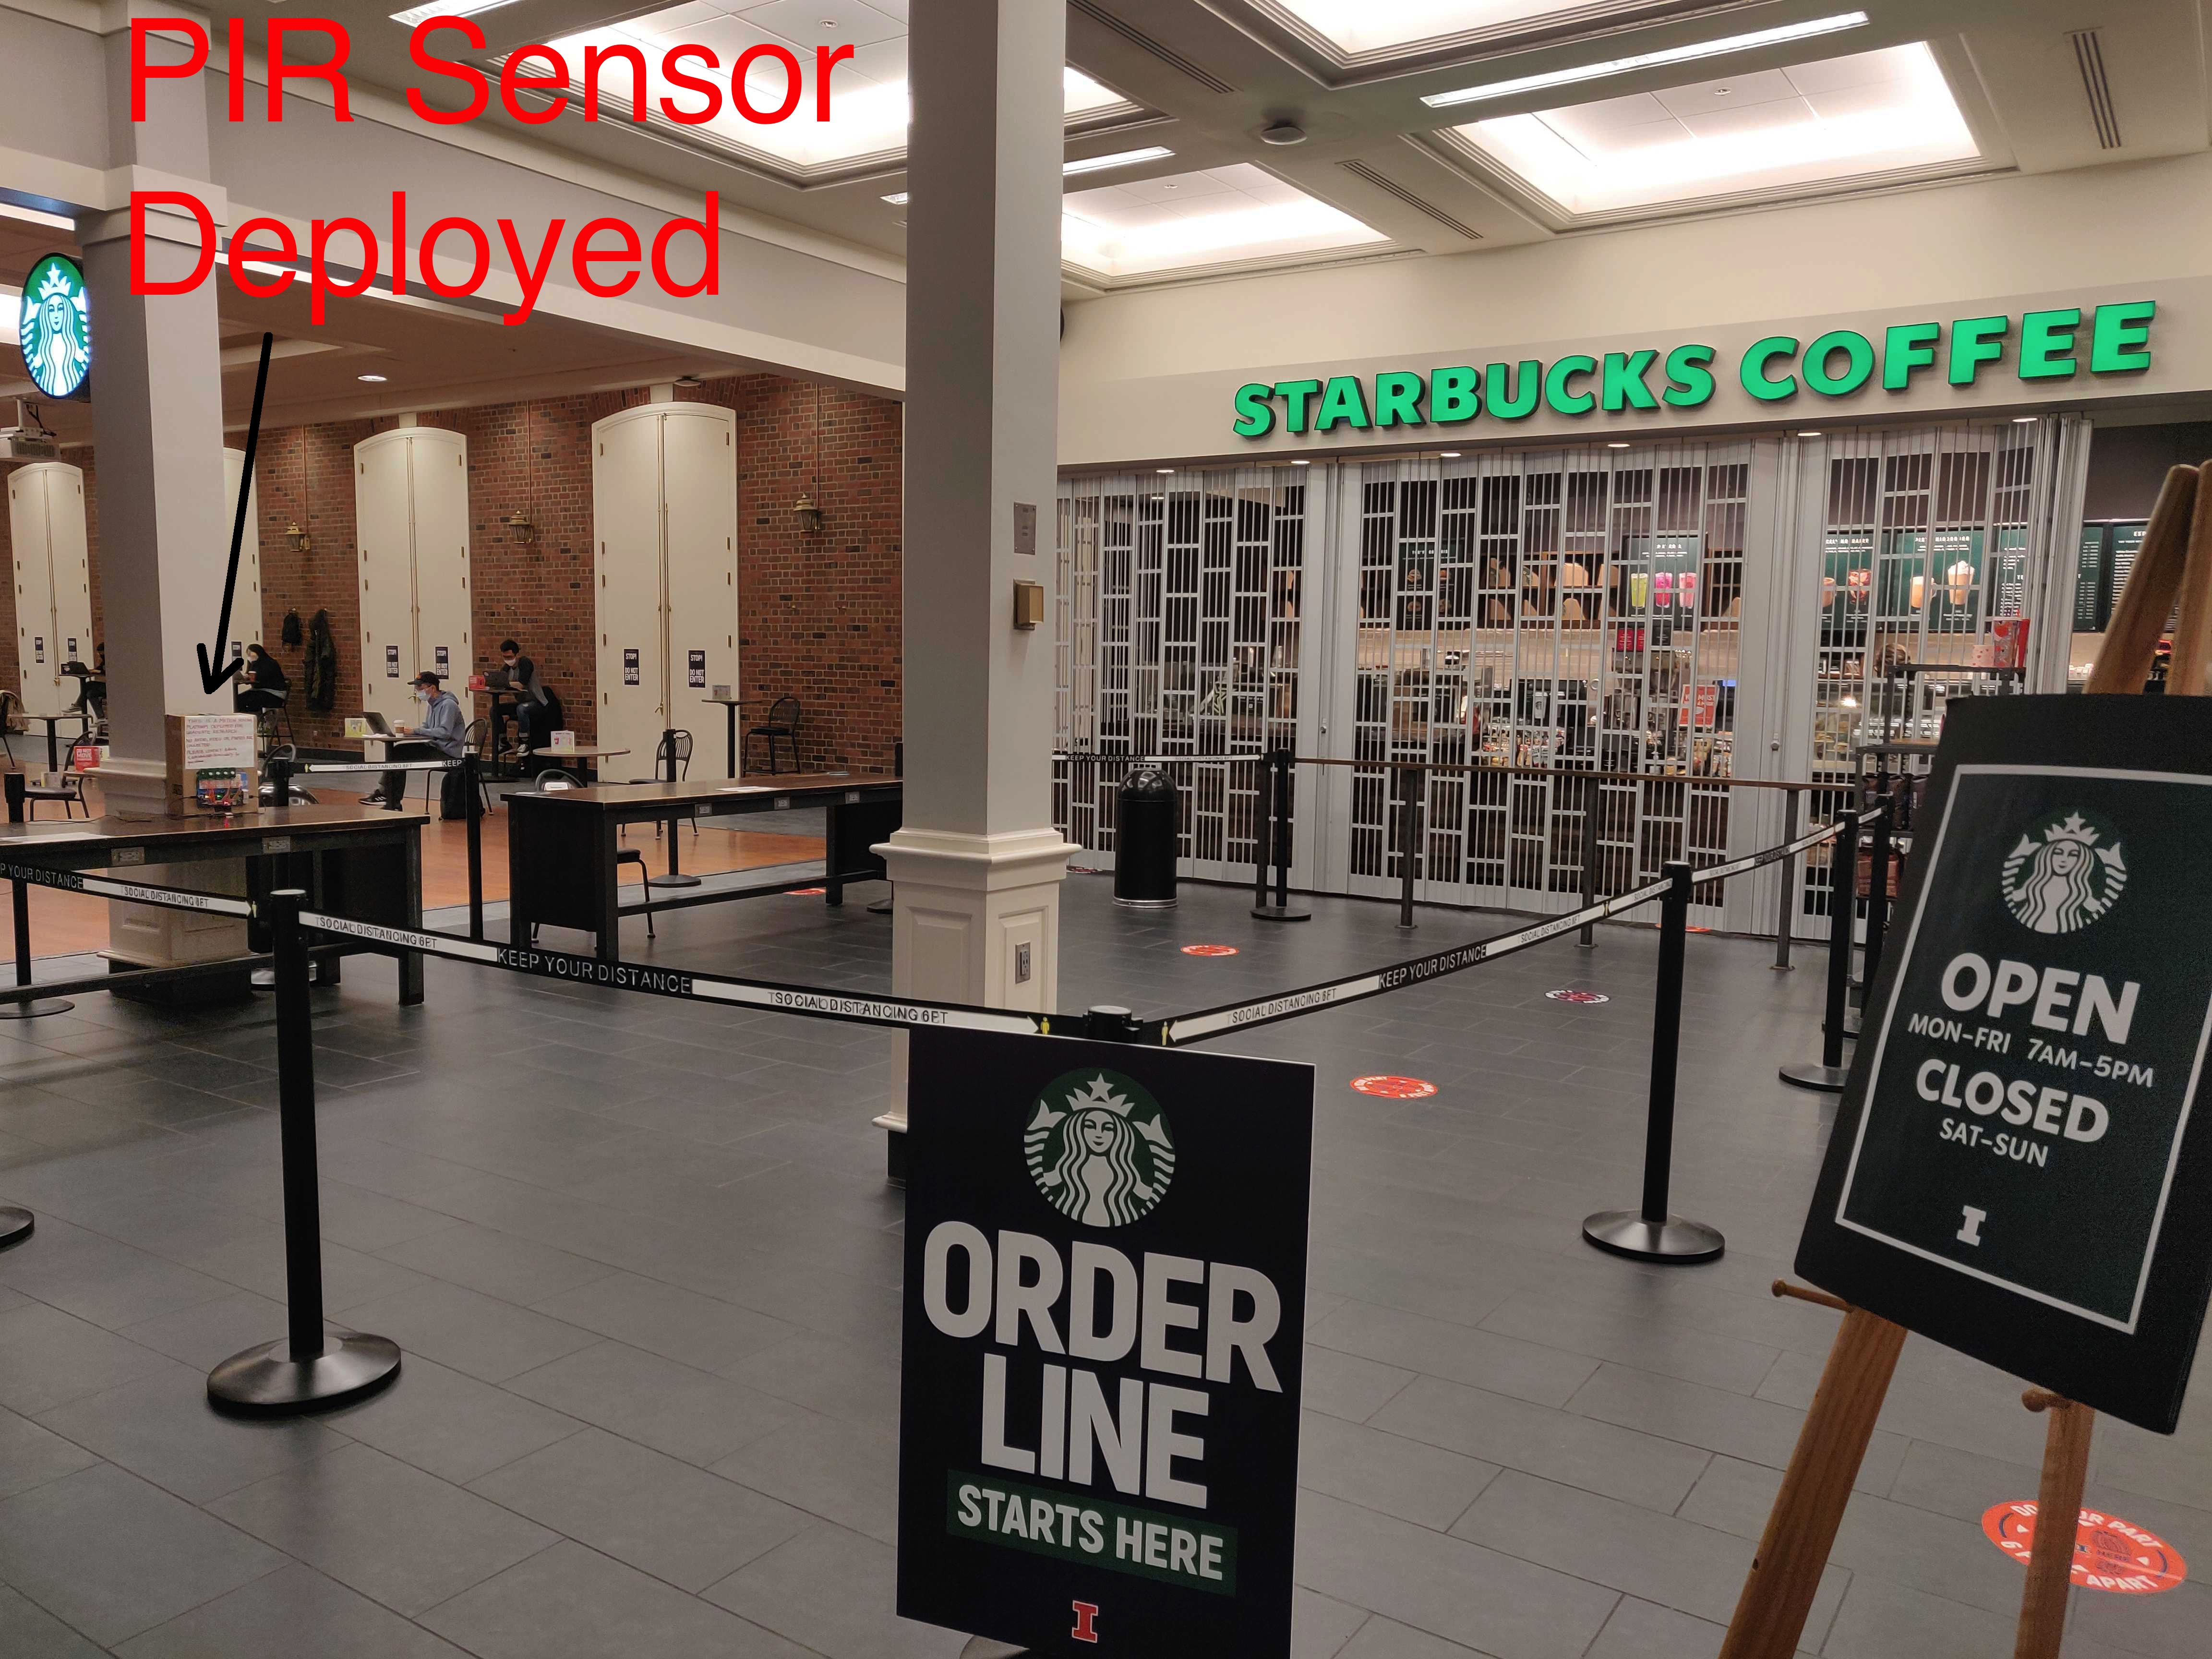
\includegraphics[width=0.3\textwidth]{figures/deployment/coffee_shop/Starbucks-jpg.jpg}
	\caption{\footnotesize{Deployment Scenarios} used for evaluating \sol in PIR sensor failure detection and diagnosis~\viz Elevator, Lobby of a building and Starbucks coffee shop.}
	\label{fig:pir_deployment_scenario}
\end{figure}
\begin{figure*}
    \begin{subfigure}[t]{0.4\textwidth}
        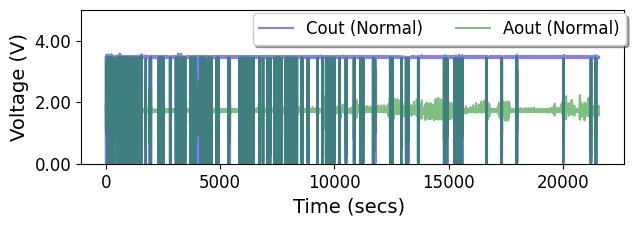
\includegraphics[width=\textwidth]{figures/deployment/elevator/afternoon-6hr.png}
    	\caption{}
    	\label{fig:deployment_csl_elevator}%
	\end{subfigure}\hfill%
	\begin{subfigure}[b]{0.59\textwidth}
	    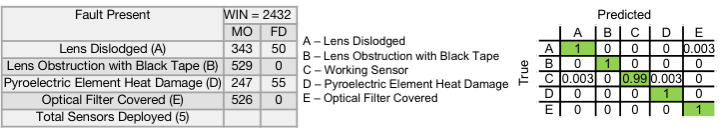
\includegraphics[width=\textwidth, height=0.65in]{figures/deployment/elevator/confusion-matrix-elevator-camera-ready.png}
		\caption{}
		\label{fig:elevator_classification_results}
	\end{subfigure}%
\caption{\footnotesize Elevator Deployment \ca Occupancy : The graph is a 6 hour deployment during business hours, \cb Deployment Statistics and confusion matrix of the classification model. Column titles: \textbf{WIN}$\rightarrow$Total Number of Windows, \textbf{MO}$\rightarrow$Misses Obstacle, \textbf{FD}$\rightarrow$ False Detection.}
\end{figure*}
\begin{figure*}
	\centering
	\begin{subfigure}[t]{0.4\textwidth}
		\centering
		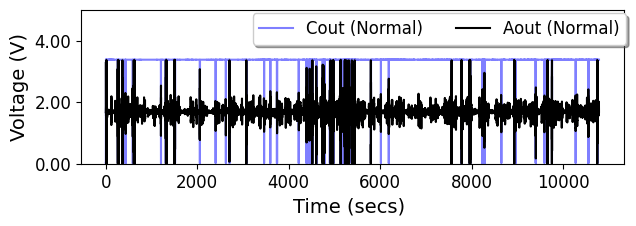
\includegraphics[width=\textwidth]{figures/deployment/lobby/lateafternoon-3hrs.png}
		\caption{}
        \label{fig:deployment_csl_lobby}%
	\end{subfigure}\hfill%
	\begin{subfigure}[b]{0.59\textwidth}
	    \centering
	    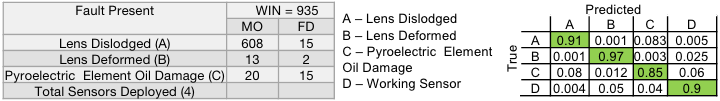
\includegraphics[width=\textwidth]{figures/deployment/lobby/confusion-matrix-lobby-camera-ready.png}

	    \caption{}
	    \label{fig:lobby_classification_results}
	\end{subfigure}
	\caption{\footnotesize Lobby Deployment \ca Occupancy graph during late evening from 6.45 pm to 9.45 pm at the lobby of our university building, \cb Deployment Statistics and confusion matrix of the classification model. Column titles: \textbf{WIN}$\rightarrow$Total Number of Windows, \textbf{MO}$\rightarrow$Misses Obstacle, \textbf{FD}$\rightarrow$ False Detection.} 
\end{figure*}
\begin{figure*}
	\begin{subfigure}[t]{0.4\textwidth}
		\centering
		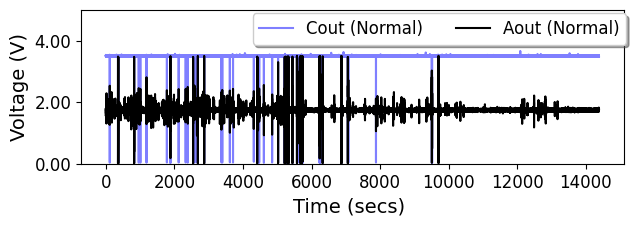
\includegraphics[width=\textwidth]{figures/deployment/coffee_shop/starbucks_4hr_deployment.png}
		\caption{}
		\label{fig:deployment_starbucks}
	\end{subfigure}\hfill%
	\begin{subfigure}[b]{0.59\textwidth}
	    \centering
	    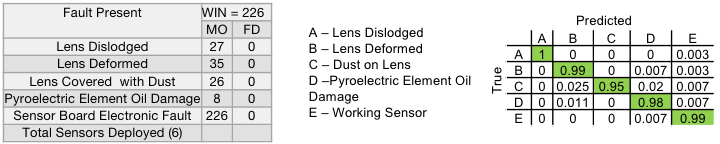
\includegraphics[width=\columnwidth]{figures/deployment/coffee_shop/confusion-matrix-coffeeshop-camera-ready.png}
	    \caption{}
	    \label{fig:coffeeshop_classification_results}
	\end{subfigure}
	\caption{\footnotesize \textbf{Starbucks Deployment Occupancy}: Evening deployment from 4.45 pm to 8.45 pm. The second half has much lesser little foot traffic. \cb Deployment Statistics and confusion matrix of the classification model. Column titles: \textbf{WIN}$\rightarrow$Total Number of Windows, \textbf{MO}$\rightarrow$Misses Obstacle, \textbf{FD}$\rightarrow$ False Detection. }
\end{figure*}


\subsubsection{Deployment in a University Elevator (US)}\label{subsubsec:elevator} 
We deployed working and faulty sensors along the inside wall of an elevator in our university research building (middle {\bfseries Fig.~\ref{fig:pir_deployment_scenario}}). 
The data collection captured scenarios of both high and low occupancy during and outside of business hours. %
In addition to faulty sensors, we placed a normal, working sensor to keep track of the actual motion in the elevator. 
{\bfseries Fig.~\ref{fig:deployment_csl_elevator}} plots \cout and \aout values captured by the working sensor showing the actual traffic in the elevator on one of the days.%
Vertical stripes on the graph showing oscillations of \cout (in blue) are points of occupancy \ie denoting a person's entry/exit at the elevator. Likewise, regions of graph with no occupancy is represented by a flat line, hovering around 3.7 V. 

\newcommand{\elevatortable}{%
		\footnotesize
		\centering
		\begin{tabular}{ | l | c | c | }
			\hline
			\multirow{2}{*}{\bfseries \textsc{Fault Present}} & 
			\multicolumn{2}{c|}{\bfseries WIN = 2432} \\
			\cline{2-3}
			& \bfseries MO &  \bfseries FD \\ \hline \hline
			Lens Dislodged &  343 & 50   \\ \hline
			Lens Covered with Black Tape &  529 & 0   \\ \hline
			Pyroelectric Element Heat Damage &  247 &  55 \\ \hline
			Optical Filter Covered & 526 & 0  \\ \hline
			Sensor Board Short & 529 & 0 \\ \hline
		\end{tabular}			
}




For faulty sensors, we measure the number of time windows where an obstacle was captured or missed. 
The performance of faulty sensors relative to a working sensor is tabulated in {\bfseries Fig.~\ref{fig:deployment_csl_elevator}}. 
When the lens cap is dislodged, it misses obstacles in 343 time windows whereas the (thermal) breakage of the pyroelectric element results in 247 misses. 
Overall, we observe that missed obstacles are more common than false alarms.
This ties into common observations in conference rooms operated with PIR sensor-controlled lighting, where lights turn off even with occupants present.


As described in \S\ref{subsec:high_level_algorithm}, \sol collects the \aout signals and uses a machine learning model on their extracted features detect faulty sensors. %
Using a random forest classifier, we obtain the confusion matrix ({\bfseries Fig.~\ref{fig:elevator_classification_results}}), which shows that predicted label matches the true label for each failure. 
We note that -- \ca the working sensor has distinct characteristics compared to the faulty sensors and is isolated correctly, \cb faulty sensors with different failures in lens and pyroelectric subsystem are identified to the failure class correctly as observed by diagonal of the confusion matrix. This implies that the %
features of \aout, derived by \sol is able to differentiate between lens being dislodged, lens being covered with tape, oil condensation on the optical filter and heat damage on the pyroelectric element.



\subsubsection{Deployment in a University Lobby (US)}\label{subsubsec:lobby} We deployed our sensors %
in the first floor lobby space of our university building. 
The lobby deployment is noisier with fewer constraints on direction of motion, compared to the confined space of an elevator.
As in the elevator deployment, we deployed a combination of working and faulty sensors shown in the table in {\bfseries Fig.~\ref{fig:lobby_classification_results}}. 



\textbf{Fig.~\ref{fig:deployment_csl_lobby}} shows a 3 hour slice of the deployment. %
The vertical stripes on \cout correspond to traffic entering/exiting the lobby in the field of view. 
The performance of the sensors deployed, in terms of false detection and missed obstacles, is shown in the table in {\bfseries Fig.~\ref{fig:lobby_classification_results}}. The sensors with lens dislodged missed a large amount of obstacles. This is due to the lack of focus of thermal radiation on the pyroelectric element resulting in dispersion of radiation due to the large lobby area. As a result of this failure, only obstacles that line up in the reduced field of view, are captured. This issue is not present in an elevator due to its confined space.
Other faults such as lens deformation and damage due to oil condensation experienced lesser number of misclassifications. 
Upon extracting the features of the \aout signals, and classifying it using the procedure in \S\ref{subsec:high_level_algorithm}, %
we observe the confusion matrix as shown in {\bfseries Fig.~\ref{fig:lobby_classification_results}}. The high fraction along the diagonal shows that a majority of sensor failures are classified and identified correctly, as the features are able to bring out differences in the physics of failures.
Note that we observe some misclassifications of sensor faults (\eg for C). We argue that this is due to the deployment area of a lobby being open and the limited coverage area of the sensor, both of which can lead to imperfect capture at the periphery. Consequently, for traffic at the edges of field of view, this reduced thermal radiations could lead to some misclassifications. %

\begin{figure*}
	\begin{minipage}[t]{0.48\textwidth}
		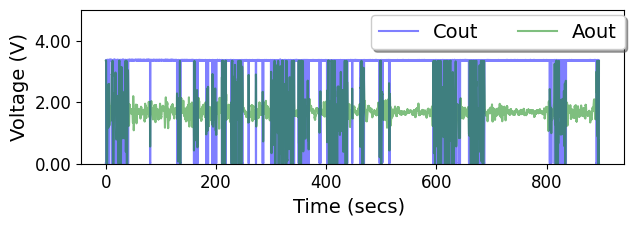
\includegraphics[width=6cm]{figures/deployment/bangalore-cafetria/msr-cafeteria-15mins.png}
		\vspace{-5pt}
		\caption{\textbf{Cafeteria Deployment occupancy} during lunchtime. A 15 min. slice of traffic at the checking counter.}
		\label{fig:deployment_msr_cafeteria}
	\end{minipage}
	\hfill
	\begin{minipage}{0.48\textwidth}
		\vspace{-\baselineskip}
		\begin{tabular}{l c c c c c}
			\hline
			\textbf{Training (MB)} & \textbf{32} & \textbf{64} & \textbf{96} & \textbf{112} & \textbf{128} \\
			\hline \hline
			Accuracy (\%) & 92.4 & 95.8 & 98.6 & 99.1 & 99.4 \\
			\hline
		\end{tabular}
		\vspace{\baselineskip}
		\caption{\textbf{Failure detection accuracy} as a function of the size of training dataset}
		\label{fig:dataset_size}
	\end{minipage}
\end{figure*}%

\subsubsection{Deployment in a Starbucks (US)}\label{subsubsec:starbucks}
We deployed PIR sensors near the ordering queue of the coffee shop during business hours to capture the typical foot traffic (left {\bfseries Fig.~\ref{fig:pir_deployment_scenario}}).
Our deployment %
captured linear, regularized bidirectional movement (entry followed by exit of the region of interest) ({\bfseries Fig.~\ref{fig:deployment_starbucks}}).
Our deployment lasted for a duration of 4 hours on a busy Friday evening.
We observed that out of 226 time windows (each containing 1024 samples), there were missed obstacles across: \ci 27 windows in class I, \cii 35 windows in class II, \ciii 26 windows in class III and no windows in class IV. The missed obstacles and false detection (none in this case) are summarized in {\bfseries Fig.~\ref{fig:coffeeshop_classification_results}}.
Using \sol, we observe high fractions along the diagonal of the confusion matrix; hence the predicted label of sensor failure matches the true label.

Furthermore, despite the oil impurity not being enough cause it to alter performance, we still classify it is a separate class from the physics point of view due to its different behavior of \aout from that of a working sensor.
Thus, in line with the previous deployments, we can use the features of \aout to form a signature of the physics. %

\begin{figure}%
	\centering
	\begin{subfigure}[t]{0.33\linewidth}
		\centering
		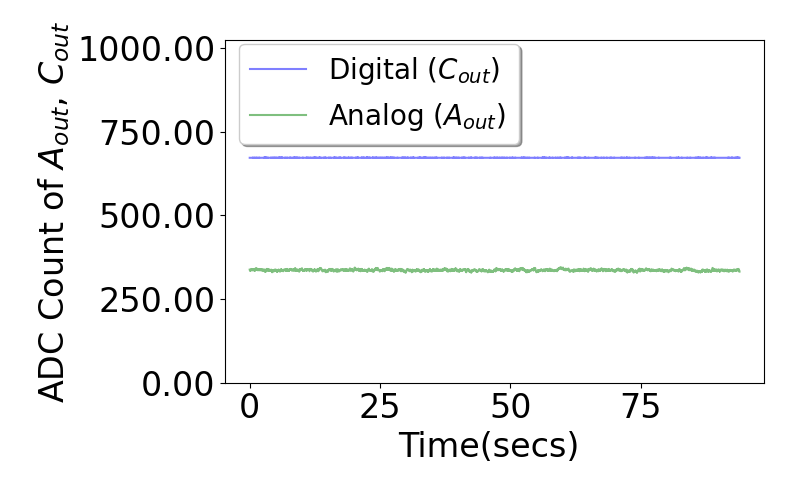
\includegraphics[width=\textwidth]{figures/pir/lens_fault/BuildSys_Graphs/CapCovered_NoObstacle.png}
		\caption{Lens Covered Completely}
		\label{fig:capcovered}
	\end{subfigure}
	\begin{subfigure}[t]{0.33\linewidth}
		\centering
		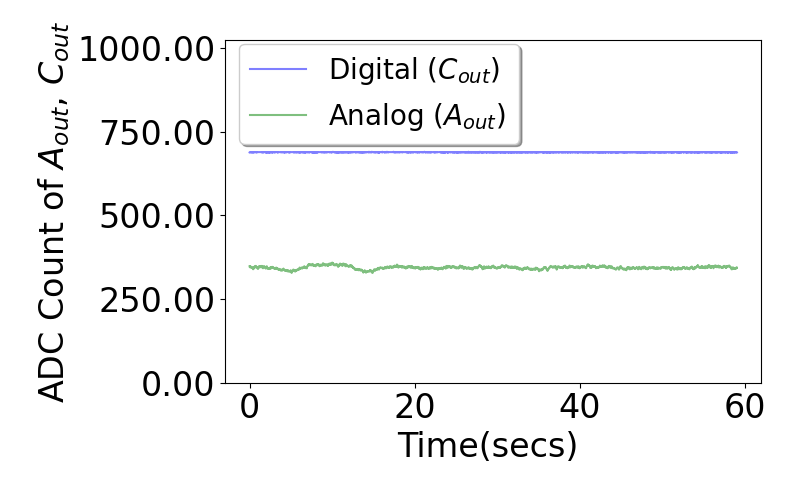
\includegraphics[width=\textwidth]{figures/pir/lens_fault/BuildSys_Graphs/CapON_NoObstacle.png}
		\caption{Lens in Place (Working)}
		\label{fig:capon}
	\end{subfigure}
	\begin{subfigure}[t]{0.33\linewidth}
		\centering
		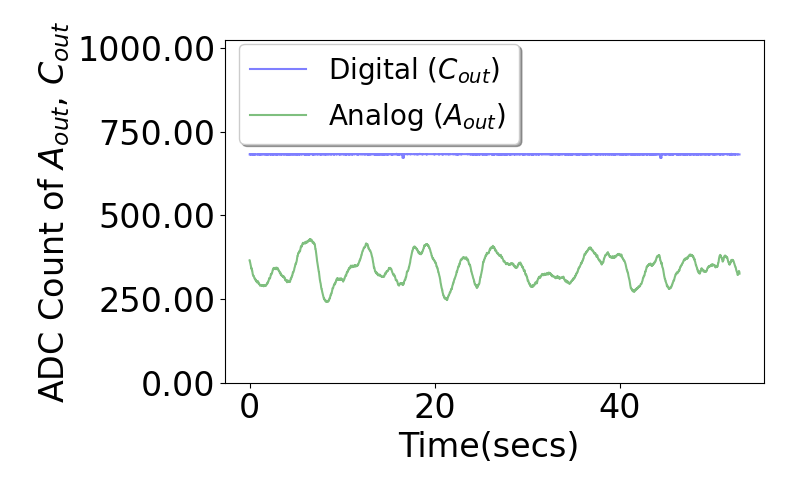
\includegraphics[width=\linewidth]{figures/pir/lens_fault/BuildSys_Graphs/CapOff_NoObstacle.png}
		\caption{Lens Dislodged}
		\label{fig:capoff}
	\end{subfigure}
	\caption{The variance in \aout during known quiet times contains hints about lens failures in the PIR sensor.}
	\label{fig:variance_cap_cases}
\end{figure}

\subsubsection{Deployment in a Cafeteria}\label{subsubsec:cafeteria} To evaluate the analysis of \aout during quiet times, we deployed a mix of 3 types of sensors with lens failures -- lens fallen off, lens covered and some working sensors during the lunch hour at a cafeteria in India. The traffic during lunchtime in the cafeteria is as shown in {\bfseries Fig.~\ref{fig:deployment_msr_cafeteria}}. As these were lens-related failures, we looked at the time-domain characterization of \aout during quiet times to understand the status of lens. The time domain representation of \aout, during a period of no occupancy, is as shown in {\bfseries Fig.~\ref{fig:variance_cap_cases}}. The y-axis is plotted in terms of the 10-bit ADC representations of voltage to highlight the differences. For a 10-bit ADC, 1023 units (\ie $2^{10} - 1$) corresponds to a voltage of 5 V. Therefore, a voltage of 1.8 V corresponds to 340 units.

We note visually that the noise floor at output of the lens subsystem is higher with the lens dislodged ({\bfseries Fig.~\ref{fig:capoff}}) as compared to both a normal sensor ({\bfseries Fig.~\ref{fig:capon}}) and one with lens covered ({\bfseries Fig.~\ref{fig:capcovered}}). Specifically, we observed a variance of 10 $Volt^2$ when lens was covered, 250 $Volt^2$ when lens was in place and working, and 1500 $Volt^2$ when lens had fallen of completely. Consequently, a low threshold ($T_L$) of 100 $Volt^2$ and a high threshold ($T_H$) of 1000 $Volt^2$ was sufficient to separate between the 3 types of sensors. Note that the variance had to be computed during a quiet period of no traffic in this case. %

We now discuss the different stages of \sol, as enumerated in the beginning of this section. 

\subsection{Stage I -- Failure Detection}
\label{subsec:fail_detection}

We aggregated all the sensors (both working and faulty) to \textit{separate faulty sensors (without specifying which class) from working sensors}. 
We collected FFT coefficients of \aout on a pre-deployment lasting 1 week and performed daily collection of \aout signals from all the deployed sensors. 
We used a Random Forest classifier with specifications shown in {\bfseries Fig~\ref{fault_detection_results}}. 
Once predicted, we manually verified the true status of the sensor and observed an accuracy of over 99\% in predicting if the sensor is working or faulty. 
Thus, FFT-based features of \aout were able to capture the physics, and hence separate faulty sensor physics from working sensor physics.
We also varied the \textit{size of training dataset} (128 MB corresponds to 1 week pre-deployment) to show the robustness of failure detection in {\bfseries Fig.~\ref{fig:dataset_size}}.


\begin{wrapfigure}{lr}{0.5\textwidth}
	\centering
	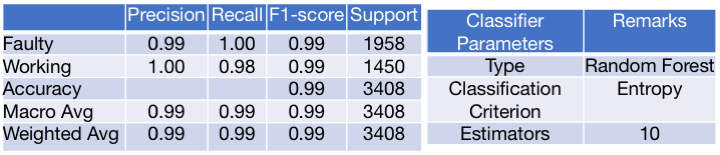
\includegraphics[width=0.5\textwidth]{figures/classification/FaultDetectionResults.png}
	\caption{\footnotesize Fault Detection showing that faulty sensors isolated from working sensors by extracting FFT of \aout and using a Random Forest Classifier.}
	\label{fault_detection_results}
\end{wrapfigure}